%! Author = chrystal
%! Date = 25.11.19

% Preamble
\documentclass[11pt]{article}

% Packages
\usepackage{amsmath}

\chapter{Data Classification}

\section{Definitions}

\subsection{Biases}

\paragraph{Third-variable Problems}describe Problems, in which a third unfocused variable is responisble for a causality
(e.g. corretlation between icecream consumption and number of drwonings).

\paragraph{Selection Bias} describes a bias caused by a subjective, unrepresentative selection of target groups for a study.

\subsection{Conditional Probability}

\paragraph{Example: Conditional Probability} For a specific serious disease, the proportion of the population found to have the disease is 10 out of 1000 persons.
You can do a screening test. If you indeed have the disease, then the test will be positive with a probability of 90\%; If you do not have the disease, then test will be positive with a probability of 9\% (false positive).
What is the Probability of being ill, if you have a positive test score? \textbf{Solution}: $P(Ill|Positive) = \frac{9}{98,1} = 0,092$.\\

\begin{tabular}{ l c c c }
    & Ill & Not ill & Sum \\
    Positive Test & 9 & 89,1 & 98,1 \\
    Not Positive Test & 1 & 900,9 & 901,9 \\
    Sum & 10 & 990 & 1000 \\
\end{tabular}

\subsection{Variable Types} \\
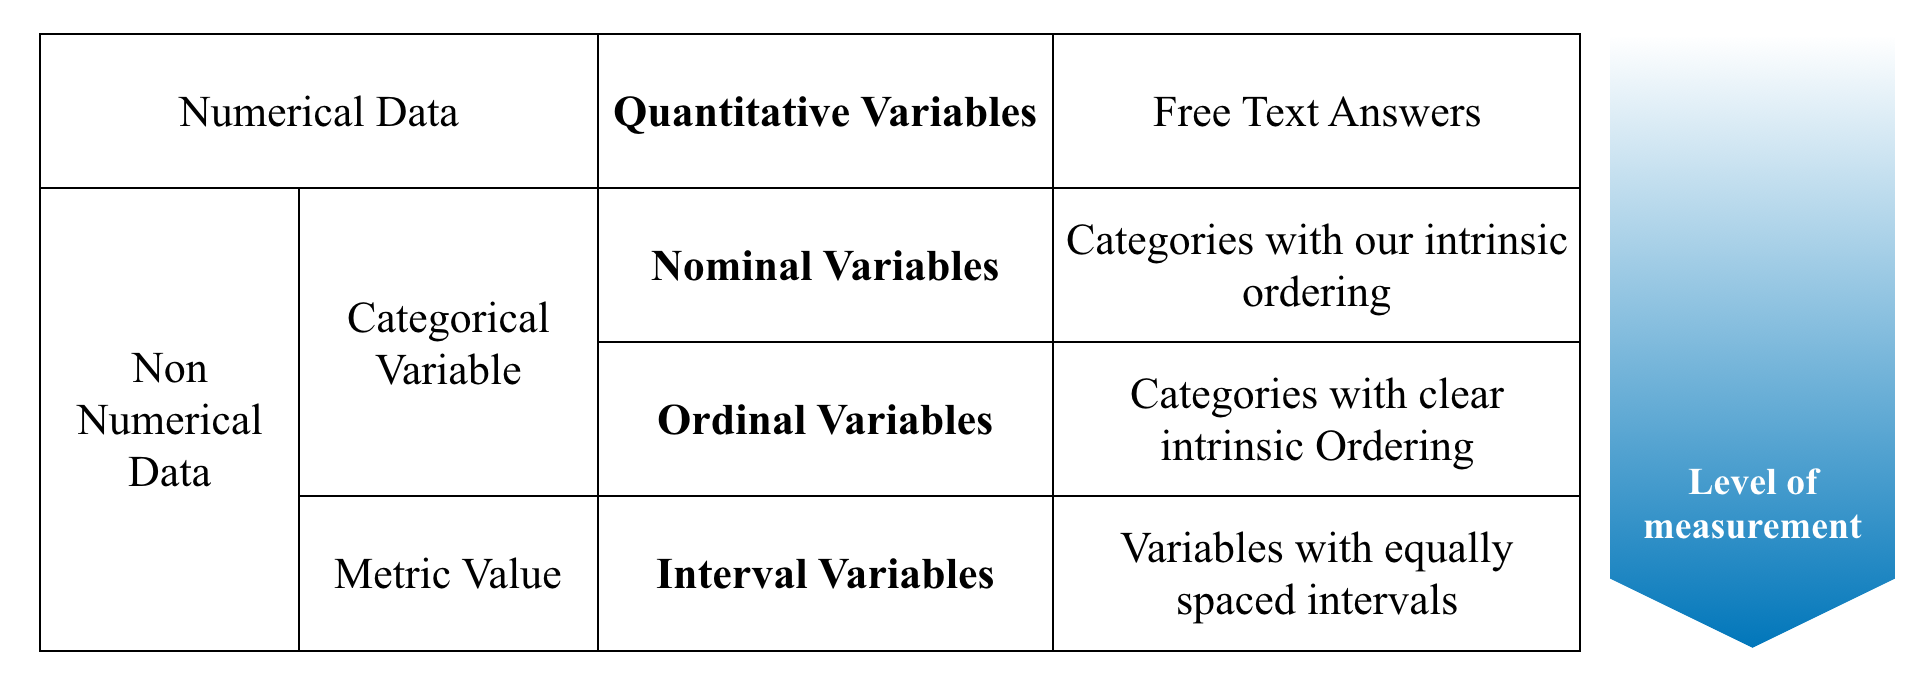
\includegraphics{../assets/variable-types.png}

\paragraph{Questionnaire Design} \textbf{A questionnaire is a set of questions for obtaining information needed for a specified goal of a certain target group}. 
A questionnaire should start with some information and a consent sheet, maybe followed by \textbf{screening questions} to filter out non-fitting candidates. Only necessary, non-leading questions, without double barreling should be asked. 
\textbf{Filter questions} may determine how good the participant is informed about the subject. 
To overcome unwillingness to answer sensible topics should be placed in the end, use third-person formulation, provide response categories. Define questions in terms of who, what, when, where. 
\textbf{Pretesting} refers to the testing of the questionnaire on a small sample of respondents to identify and eliminate potential problems

\subsection{Scaling Techniques}

A scaling technique is a procedure to investigate the preferences of a respondent to objects regarding one or multiple characteristics.

\begin{tabular}{  p{1.5cm}  p{3cm}  p{3cm}  p{3cm}  }
    &  \textbf{Respondents task} & \textbf{Limitations} & \textbf{Data Interpretation} \\
    \hline
    \multicolumn{4}{c}{\textbf{Comparative Scaling}} \\
    \hline
    Paired Comparison \newline (ordinal) &
    Respondents are presented with 2 objects and asked to select one &
    Requires $n(n-1)/2$ comparisons per person for n brands &
    Showing each brand against every other in a table, with x dimensional sum, filled with the percentage of participants enjoying one over the other.  \newline \\

    Rank Order \newline (ordinal) &
    Respondents are presented with several objects simultaneously and asked to rank them  \newline &
    It is possible that the respondent may dislike the first ranked &
    Looking at the distribution of ranks for the different criterion's separately \\

    Constant Sum \newline (ordinal) &
    Respondents allocate a constant sum of units, such as 100 points to attributes of a product to reflect their importance &
    Tend to reduce halo or carryover effects from one judgment to another. It comes with the inability to generalize beyond the stimulus objects scaled. \newline &
    \\

    \hline
    \multicolumn{4}{c}{\textbf{Non-omparative Scaling}} \\
    \hline
    Likert \newline (ordinal) &
    Rrespondents indicate the extent to which they agree or disagree with a series of statements about the object &
    Might cause Order effect, Central tendency, Pattern answering. Usage of balanced or balanced, even or odd, forced or nonforced, verbal description categories, continuous rating? \newline &
    item-by-item basis (profile analysis) or a total score (mean) \\

\end{tabular}

\section{Marketing Research}

\paragraph{Marketing Research} Marketing research is the systematic and \textbf{objective, identification, collection, analysis, dissemination},
and use of information for the purpose of improving decision making related to the identification and solution of problems and opportunities in marketing.
We want to know what consumers do, think and feel – Information to identify opportunities and refine and evaluate actions.

\subsection{Research Types}

\begin{tabular}{ p{5.5cm} p{6cm} }
    \textbf{Segmentation Research}
    \begin{itemize}
        \item Determine the basis of segmentation of markets
        \item Establish market potential and responsiveness for various segments
        \item Create lifestyle profiles: demography, media, and product image characteristics
    \end{itemize}
    &
    \textbf{Product Research}
    \begin{itemize}
        \item Test concept to determine optimal product design
        \item Package tests or Control score tests with Product modification
        \item Brand positioning and repositioning
    \end{itemize}
    \\
    \textbf{Pricing Research}
    \begin{itemize}
        \item Researches importance of price in brand selection
        \item Price elasticity of demand to Initiating and responding to price changes
    \end{itemize}
    &
    \textbf{Promotional Research}
    \begin{itemize}
        \item  Evaluation of advertising effectiveness to find the optimal promotional budget and promotional mix
        \item Creative advertising testing
        \item Claim substantiation
    \end{itemize}
    \\
\end{tabular}

\subsection{Research Procedure}

\paragraph{1. Problem Definition} Management Decision Problem (action oriented) \textit{E.g. Should a product be introduced} $\leftrightarrow$ Marketing research problem (provide infos for management problem) \textit{E.g. What are the consumer preference and purchase intent?}. Research Problems need to consider Past information (Market, sales, demographics), Resource constraints (Cost and timing), Objectives, Buyer behavior (Demographics, consumption habit, price sensitivity), Legal constraints, Economic environment (Income and purchasing power), Technological constrains.\\

\textbf{2. Research Design} \newline

\begin{tabular}{  p{1.5cm}  p{3cm}  p{3cm}  p{3cm}  }
    &  \textbf{Exploratory}     & \textbf{Descriptive}   & \textbf{Explanatory / Conclusive} \\
    Variables
    & no known Variables
    & Defined Variables
    & Defined Variables and Relationships \\
    Objective
    & Discovery of ideas and insights
    & Describe market characteristics or functions
    & Determine cause and effect relationships \\
    Characteristics & Often the front end of total research design
    & Prior formulation of specific hypotheses; Preplanned and structured design
    & Manipulation of one or more independent variables \\
    Objective
    & Expert surveys, Pilot surveys, Secondary data (qualitative)
    & Secondary data: quantitative analysis, Surveys, Observation
    & Experiments \\
    Sampling
    & Non-probability Sampling
    &
    & Probability Sampling
\end{tabular}

\paragraph{3. Data Collection} \textbf{Primary data} is Data that are directly collected for the purposes of the research under the researcher’s control. \textbf{Secondary data} Data that is gathered by someone else (for a purpose other than that which the researcher has in mind).

\paragraph{4. Analysis}

\paragraph{5. Report and presentation}
